\documentclass[3p, twocolumn, number, a4paper, 10pt, oneside, preprint]{elsarticle}

\usepackage[square]{natbib}
\usepackage{graphicx}
\usepackage{scrtime}
\usepackage[automark]{scrpage2}
\usepackage{amsmath}

\pagestyle{scrheadings}

\newcommand{\geant}{\textsc{Geant4} }

\journal{Computer Physics Communication}

\begin{document}

\begin{frontmatter}

\title{Integrating Tracking and  Beam-Matter-Interaction for Beam line Design}

\author[fzd]{L. Clemente\corref{cor}}
\ead{l.clemente@fzd.de}
\author[fzd]{M. Bussmann}

\cortext[cor]{Corresponding author}
\address[fzd]{Forschungszentrum Dresden-Rossendorf, Dresden, Germany}

\begin{abstract}
	Current developments in particle acceleration technologies, specifically interesting for medical applications come along with a massive reduction of space of the source. Although a complete accelerator might fit into a room, the beam line for beam transportation is still a massive system which can for reasons of radiation protection not be scaled easily.
	
	In this publication, we present a modular software tool integrating advanced particle tracing with effects like space charge and sophisticated beam matter interactions. As tracker module we use a common particle tracing algorithm, the general particle tracer (GPT), and a established beam matter interaction simulation toolkit, Geant4, as interaction module. The algorithm is described, the software architecture explained and the code is verified in several exemplary application cases.
\end{abstract}

\begin{keyword}
	Laser Acceleration \sep Particle Tracing \sep Beam line design
	
	\PACS 41.75.Jv %Laser driven acceleration
	\sep 07.05.Fb %Design of experiments (computers)
	\sep 87.56.bd %Radiation sources (medical physics): accelerators
	\sep 41.85.-p %Beam optics (charged-particle beams)
	\sep 41.75.Ht %Beams, charged-particle, relativistic electron and positron
\end{keyword}

\end{frontmatter}



\section{Introduction}
\label{introduction}

With current advances in particle acceleration, especially laser acceleration techniques, a leading thought is to develop small medical devices, requiring only a fraction of space compared to a conventional apparatus. Applications may be x-ray diagnosis or radiation treatment (e.g. with protons). Laser sources are e.g. described in [ref], for possible applications see [ref].

One remaining challenge with small particle sources is the design of a small beam line, as large systems would annihilate the effect of space gain. Designing a compact beam line for medical purposes is a even more delicate process: The patient has to be secured from unwanted radiation, but the overall size must not exceed certain maxima. Along with the decrease of beam line size comes especially the aspect of radiation protection, which has to be taken into account during the design process.

Conventional beam lines are often designed using software packages that fit for one specific aspect. There exist advanced particle tracing algorithms for detailed simulation of particles passing electromagnetic fields and more complex processes, e.g. space charge effects. Another class of codes simulates the interaction of particles with matter	 based on physicals effect models. Building a compact beam line requires both of this aspects combined together. Secondary particles generated e.g. in pinholes may not be neglected.

We therefore developed a modular simulation tool integrating particle tracing and beam matter interaction and fulfilling these requirements. A common particle tracing algorithm can thus easily be combined with an interaction simulation tool for beam line design.

\section{Software design}
\label{design}

\subsection{Structure}
\label{structure}

The simulation toolkit flint (\underline{F}ZD \underline{L}aser \underline{In}teractor and \underline{T}racker) consists of two main modules, a "tracker" and an "interactor". An interface between both at stepping level is established and both modules are used for calculation of a particles trajectory, secondaries, etc. The user has thus access to all elements of both modules. In particular, this means tracking massive amounts of particle through complex geometries and fields, considering effects like space charge on the tracker side or e.g. fission on the interactor side.

\subsection{The combination of GPT and \geant}
\label{combination}

There are only few limitations to a tracker or interactor to be fitted into flint. In this paper we use GPT [ref] as tracker and Geant4 [ref] as interactor, but other combinations would be possible with little effort as well. Both tools fulfil all requirements for successful integration.

\subsection{Integration into the tracker}
\label{integration}

The interface between GPT and Geant4 is provided by a GPT custom element, which calls the Geant4 if necessary. This custom element would also be easily integratable into other trackers. Basically every tracker step is performed as usual. After every step, the software check every particle's trajectory for intersection with an interactor solid. The pre and the post step point of the tracker are considered. Afterwards the interactor is used to recalculate the step and the results are reinjected as shown in \ref{stepping}. After this process some detailed output is written. Then, the tracker continues normally.

\subsection{Combined stepping}
\label{stepping}

In the following, we will describe the exchange of information between the tracker and the interactor for one particle:

\begin{enumerate}[1.]
	\item A step is tracked normally by GPT, using information about all other particles in the simulation.
	\item The step is recalculated individually for each particle using Geant4.
		\begin{itemize}
			\item A particle is generated and started at the pre tracker point, facing with tracker post velocity in direction of the tracker's post step point (thus flying as a secant).
			\item The calculation stops, when the stepping time of the tracker is exceeded.
		\end{itemize}
	\item Reinjection of the results from the interactor to the tracker.
		\begin{itemize}
			\item The new position and velocities are taken directly.
			\item The rotation of momentum between pre interactor and post interactor is calculated.
			\item The post tracker momentum is rotated accordingly.
		\end{itemize}
\end{enumerate}

An example step to illustrate the stepping algorithm is shown in Figure \ref{fig_stepping}.

\begin{figure}
	\centering
	\includegraphics[width=0.55\columnwidth, page=7]{img/stepping}
	\caption{An illustration of the stepping algorithm}
	\label{fig_stepping}
\end{figure}

Secondaries produced during the interaction calculation are differentiated by mass and charge. Massless or uncharged particles are exclusively tracked by the interactor and not reinjected to the tracker as most trackers can not handle these. All other particles are added normally to the tracker's particle set.


\subsection{Input for the calculation}
\label{input}

The definition of the calculation world of flint takes place in one single place, a XML file. This file basically has two parts, one for defining tracker options and on for defining the geometry, processes and particles to be used by the interactor. Flint also includes a tool for visualising geometries defined by this XML file. An exemplary visualisation of a geometry can be seen in [ref].

\subsection{Output}
\label{output}

Flint currently includes several output options. Of course, all output of the tracker and interactor can be used. Flint also provides some additional options like unified trajectories of all particle types (including massless and uncharged particles) or energy deposition in the geometry. This output is written as ASCII, macros for gnuplot [ref] visualisation are provided.

\subsection{Parallisation}
\label{parallisation}

Parallelising a tracker is often a very difficult process. In the interactor part though, all particles are handled independent from each other, not interfering. This is why flint parallelises the interactor and, additionally the output module. Parallisation is performed using OpenMP [ref] and results in significantly faster simulation.

\section{Verification and Examples}
\label{verification}



\section{Outlook}
\label{outlook}



\section{Old stuff}

\subsection{Integration into GPT}

The interface between GPT and \geant is provided by two GPT custom elements. The element \texttt{G4Virtual} has to be instantiated once in a calculation and is responsible for initializing MPI and the save termination of all \geant processes. The second custom element launches the interaction calculation, a quader shaped \texttt{G4Area} can be placed to use \geant calculations in a specific area. This should be used as a bounding box arround \geant solids. \textbf{ToDo: check for collisions in GPT?}

After every succesful GPT step, all particles are tested for beeing in a physical volume. If a single particle is inside a \texttt{G4Area}, its path will be recalculated. Therefore, the old partcle position before the step, the particle's current position, its velocity's norm in the end of the track, its mass and charge are sent to \geant. In the interactor process, the particle type is recognized by analysis of the sent particle's mass and charge. A similar particle is then started at the pre step point with the post step velocity pointing in direction of the post step point. Thus, the way calculated by \geant is (if no interactions occur) a secant of the actual GPT path.

The track length specified by GPT is tracked in \geant, although processes may occur. After the needed length, the particle's new post step point and its vectorial velocity is sent back to GPT. The post step velocity's and the new post step point are set. The new vectorial velocity is not exclusively used, as the particle's track would then be error. Instead, the change of the velocity vector in \geant is calculated and added to the GPT post step vector. The angel in between the \geant start vector $\vec{p}_{G4 old}$ and the \geant end vector $\vec{p}_{G4 new}$ can be calcuclated using the scalar product $\varphi = \vec{p}_{G4 new} \cdot \vec{p}_{G4 old}$. The axis around which the GPT post vector $\vec{p}_{GPT old}$ has to be turned, is given by $\vec{n} = \vec{p}_{G4 new} \times \vec{p}_{G4 old}$. The new GPT vector $\vec{p}_{GPT new}$ can then be calculated as

%\begin{equation}
% \vec{p}_{GPT new} = \vec{p}_{GPT old} \cos \varphi + \vec{n} ( \vec{n}\cdot \vec{p}_{GPT old} )
% ( 1 - \cos \varphi ) + ( \vec{p}_{GPT old} \times \vec{n} ) \sin \varphi
%\end{equation}

This calculation ensures the minimal error possible.

\subsection{Parallelization}
\label{paralel}

As \geant is a monte-carlo toolkit, is can be easily parallelized. In flint, the user can specify a number of \geant processes that should be used for calculation at one time. The single GPT process then provides tasks for all \geant processes and fetches the results from the finished interactors, but has to wait for all interactors to finish before starting a new step. Thus the parallization is only profitable with very large numbers of particles. Another possibility is to launch multiple GPT processes with their corresponding \geant partners. The calculation can thus be run parallel on clusters.

\subsection{Configuration}

Large simulation and therefore large geometries require a simple, standardized method to configure a simulation and setup all parameters. flint provides the possibility to use XML-Files for that purpose. In a grammar based on GDML \textbf{Zitat einfuegen!} the geometry, all fields and some additional parameters, like the particle definitions to be loaded by the interactor, can be edited and adjusted to every calculation. A script provides GPT with a GPT ini file generated from this XML file and \geant reads the file itself. The whole simulation can thus be configured in a single file.

\begin{thebibliography}{00}

\item{Agostinelli et al.}
\item{GPT Manual}

\end{thebibliography}

\end{document}

